\documentclass[12pt, a4paper, twoside]{article}
\usepackage[utf8]{inputenc}
\usepackage[cm]{fullpage}
\usepackage{fancyhdr}
\usepackage{textcomp}
\usepackage{graphicx}

\begin{document}

\title{Relatório do Experimento 3 de OAC}
\author{
Arthur Bizzi: 13/0102636 \\
Arthur da Silveira Couto: 16/0002575 \\
Caio Albuquerque Brandão: 16/0003636 \\
Cristiano Silva Júnior: 13/0070629 \\
Leonardo Maffei: 16/0033811 \\}
\date{7 de Junho de 2017}
\maketitle

\section{Exercício 1}

A fim de comparar as simulações do MARS e de forma de onda, compilamos o programa \textit{testePIPE.s} no MARS por meio da ferramenta \textit{MIF Exporter} e geramos uma simulação por forma de onda do programa, além de analisar os dados gerados a partir do programa.

No MARS, o programa, ao ser executado, não fez nada. Contudo, ao se comentar as linhas de hazard de controle, o programa é capaz de terminar a sua execução. O resultado final dos registradores pode ser visto na figura 1.

Ao simular em forma de onda, o programa gerou a forma de onda na figura 2. Pode-se notar que eles são equivalentes olhando o resultado final do registrador \textit{PC}.

\begin{figure}
    \centering
    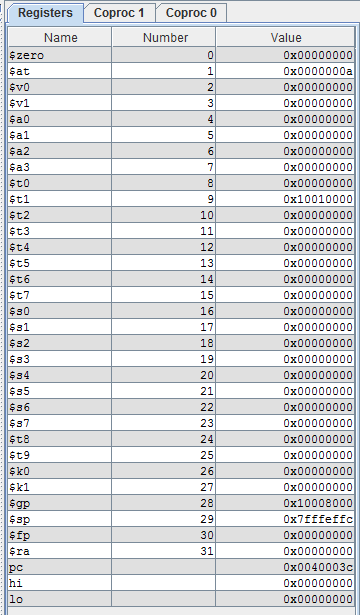
\includegraphics[width=0.8\textwidth]{./figs/testepipereg.png}
    \caption{Resultado final dos registradores .}
\end{figure}

% Como adicionar uma figura
\begin{figure}
    \centering
    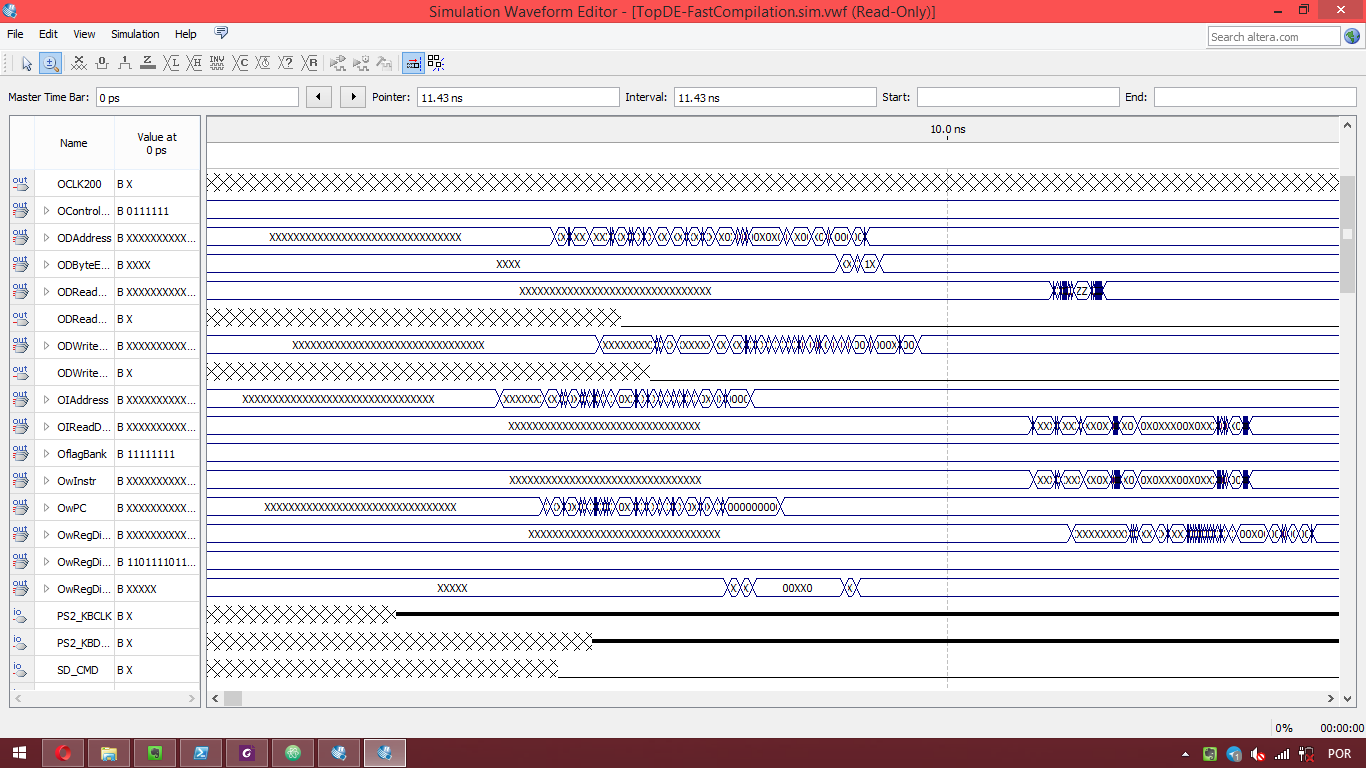
\includegraphics[width=0.8\textwidth]{./figs/simw.png}
    \caption{Simulação em forma de onda do programa \textit{testePIPE.s}.}
\end{figure}

\section{Exercício 2}

% TODO Diagrama de blocos do caminho de dados
Compilando o código em \textit{Verilog}, é possível checar o circuito gerado pelo \textit{Quartus}. A partir do circuito gerado, podemos idenfificar algumas estruturas, que estão destacadas na figura 2.

\begin{figure}
    \centering
    \includegraphics[width=0.8\textwidth]{./figs/data_pipeline.png}
    \caption{Simulação em forma de onda.}
\end{figure}

% TODO Tabela verdade da unidade de controle
Com base nessas estruturas e das ligações entre elas, podemos inferir uma tabela-verdade para o circuito de controle, como explicadas nas tabelas de 1 a 4.

\begin{table}[H]
    \centering
    \begin{tabular}{|ccccc|}
    \hline
      & OrigPC & Jump & nBranch & Jr \\
    \hline
    LW      & 0 & 000 & 0 & 0  \\
    SW      & 0 & 000 & 0 & 0  \\
    BEQ     & 0 & 001 & 0 & 0  \\
    Tipo R  & 0 & 000 & 0 & 0  \\
    J       & 1 & 010 & 0 & 0  \\
    \hline
    \end{tabular}
    \caption{Tabela de controle para estágio Decodificação da instrução}
\end{table}

\begin{table}[H]
    \centering
    \begin{tabular}{|cccc|}
    \hline
      & RegDst & OrigALU & OpALU \\
    \hline
    LW  & 00 & 01 & 00 \\
    SW  & 00 & 01 & 00 \\
    BEQ & 00 & 00 & 01 \\
    TIPO R & 01 & 00 & 10 \\
    J   & 00 & 00 & 00 \\
    \hline
    \end{tabular}
    \caption{Tabela de controle para estágio execução/cálculo de endereço}
\end{table}

\begin{table}[H]
    \centering
    \begin{tabular}{|ccccccc|}
    \hline
      & SavePC & LeMem & EscreveMem & Branch & LoadType & WriteType\\
    \hline
     LW     & 0 & 1 & 0 & 0 & LW & 00 \\
     SW     & 0 & 0 & 1 & 0 & 000 & SW \\
     BEQ    & 0 & 0 & 0 & 1 & 000 & 00 \\
     Tipo R & 0 & 0 & 0 & 0 & 000 & 00 \\
     J      & 0 & 0 & 0 & 0 & 000 & 00 \\

    \hline
    \end{tabular}
    \caption{Tabela de controle para estágio acesso à memória}
\end{table}

\begin{table}[H]
    \centering
    \begin{tabular}{|ccc|}
    \hline
      & EscreveReg & MemparaReg \\
    \hline
    LW      & 1 & \\
    SW      & 0 & \\
    BEQ     & 0 & \\
    Tipo R  & 1 & \\
    J       & 0 & \\
    \hline
    \end{tabular}
    \caption{Tabela de controle para estágio escrita do resultado}
\end{table}

% \section{Exercício 3}
%
% % TODO Analisar unidades de Hazard e Forward

\section{Exercício 4}

% TODO Simular forma de onda do programa teste.s
Repetindo o procedimento de compilação do exercício 1, podemos gerar uma simulação de forma de onda da nossa versão do programa \textit{teste.s}, contendo um breve teste de todas as funções implementadas na ISA. O resultado da simulação pode ser visto na figura 3.

\begin{figure}
    \centering
    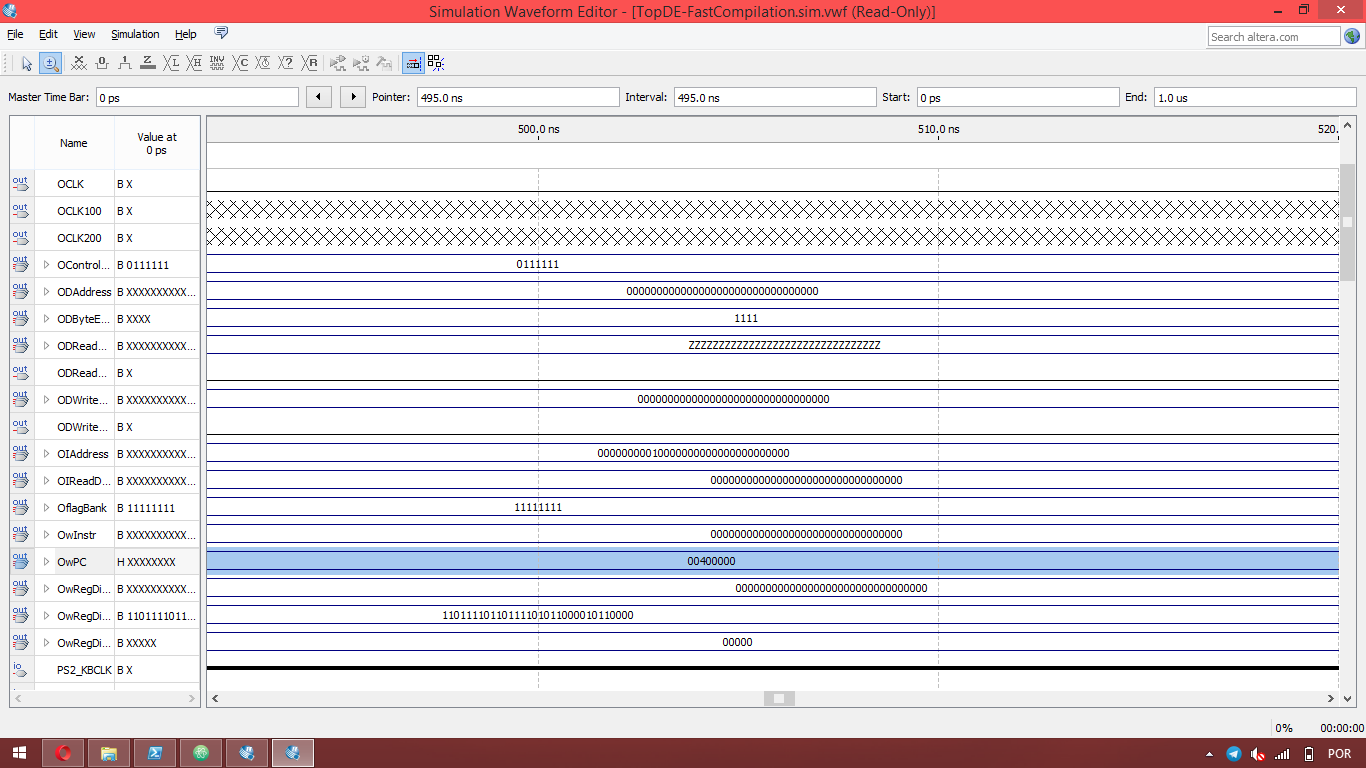
\includegraphics[width=0.8\textwidth]{./figs/sims.png}
    \caption{Simulação em forma de onda do programa \textit{teste.s}.}
\end{figure}

% \section{Exercício 5}
%
% % TODO Linkar vídeos de desenho das bandeiras
%
% \section{Exercício 6}
%
% % TODO Incluir bolhas para realizar operações de ponto flutuante
%
% \section{Exercício 7}
%
% % TODO Comparar síntese da FPULA
%
% \section{Exercício 8}
%
% % TODO Implementar ceil
% % TODO Implementar floor
% % TODO Implementar round

\end{document}
